%!TEX root = oral.tex

\section{Service Level Requirements}

	\begin{frame}
	\textbf{Paper 1: Inventory Rebalancing and Vehicle Routing in Bike Sharing Systems}
	\begin{itemize}
		\item Jasper Schuijbroek \\
		\textit{Eindhoven University of Technology}
		\item Robert Hampshire \\
		\textit{Carnegie Mellon University}
		\item Willem-Jan van Hoeve \\
		\textit{Carnegie Mellon University}
	\end{itemize}
	\end{frame}

    \begin{frame}{Definition}
    Let $\mathcal{S}$ represent the set of bike sharing stations. For each station $i \in \mathcal{S}$:
    \begin{itemize}
        \item $C_i$ denotes capacity of the station.
        \item Poisson process for bike drop-offs with rate $\lambda_i$
        \item Poisson process for bike pickups  with rate $\mu_i$
    \end{itemize}
    \pause
    The service level requirements at station $i \in \mathcal{S}$ are:
    \begin{eqnarray*}
        \frac{\mathbb{E}[\textrm{Satisfied pickup demands}]}{\mathbb{E}[\textrm{Total pickup demands}]} &\geq& \beta_{i}^{-} \\ \\
        \frac{\mathbb{E}[\textrm{Satisfied dropoff demands}]}{\mathbb{E}[\textrm{Total dropoff demands}]} &\geq& \beta_{i}^{+} \\
    \end{eqnarray*}
    for given $\beta_{i}^{-},\beta_{i}^{+} \in [0,1]$.
    \end{frame}

    \begin{frame}{Markov Chain Formulation}
    Each station is a $M/M/1/K$ queue with $K=C_i$. Markov Chain for inventory $S_i(t)$ is:
    
\begin{center}
\begin{tikzpicture}[->, >=stealth', auto, semithick, node distance=2cm, state/.style={circle, draw, minimum size=1.3cm, scale=0.6}]
\tikzstyle{every state}=[fill=white,draw=black,thick,text=black,scale=1]
\node[state]    (0)  		{$0$};
\node[state]    (+1)[right of=0]   		{$1$};
\node[state]    (+inf) [right of=+1] 	{$...$};
\node[state]    (+C-1)[right of=+inf]   {$C_i - 1$};
\node[state]	(+C)[right of=+C-1]		{$C_i$};
\path
(0)     edge[bend left]         node{$\lambda$}   (+1)
(+1)    edge[bend left]         node{$\lambda$}   (+inf)
        edge[bend left,below]   node{$\mu$}       (0)
(+inf)  edge[bend left]   		node{$\lambda$}   (+C-1)
		edge[bend left,below]	node{$\mu$}		  (+1)
(+C-1)  edge[bend left]   		node{$\lambda$}   (+C)
		edge[bend left,below]	node{$\mu$}		  (+inf)
(+C)	edge[bend left,below]	node{$\mu$}       (+C-1);	
\end{tikzpicture}
\end{center}
    \begin{itemize}
    	\pause
    	\item[--]$p_i(s, \sigma, t)$ = probability that inventory at station $i$ equals $\sigma$ at time $t \geq 0$ given starting inventory $s$ \\
    	\vspace{0.1in}
    	\pause
    	\item[--]$g_i(s, \sigma) = \frac{1}{T}\int_{0}^{T}p_i(s, \sigma, t) dt$ \\
	\end{itemize}
	\pause
	\textbf{Service Level Requirements:}
    \begin{eqnarray*}
        \frac{\mathbb{E}[\textrm{Satisfied pickup demands}]}{\mathbb{E}[\textrm{Total pickup demands}]} &=& 1 - g_i(s, 0) \\ \\
        \frac{\mathbb{E}[\textrm{Satisfied dropoff demands}]}{\mathbb{E}[\textrm{Total dropoff demands}]} &=& 1 - g_i(s, C_i) \\
    \end{eqnarray*}
    \end{frame}

    \begin{frame}{Service Level Requirements for Hubway}
        \begin{figure}
            \centering
            {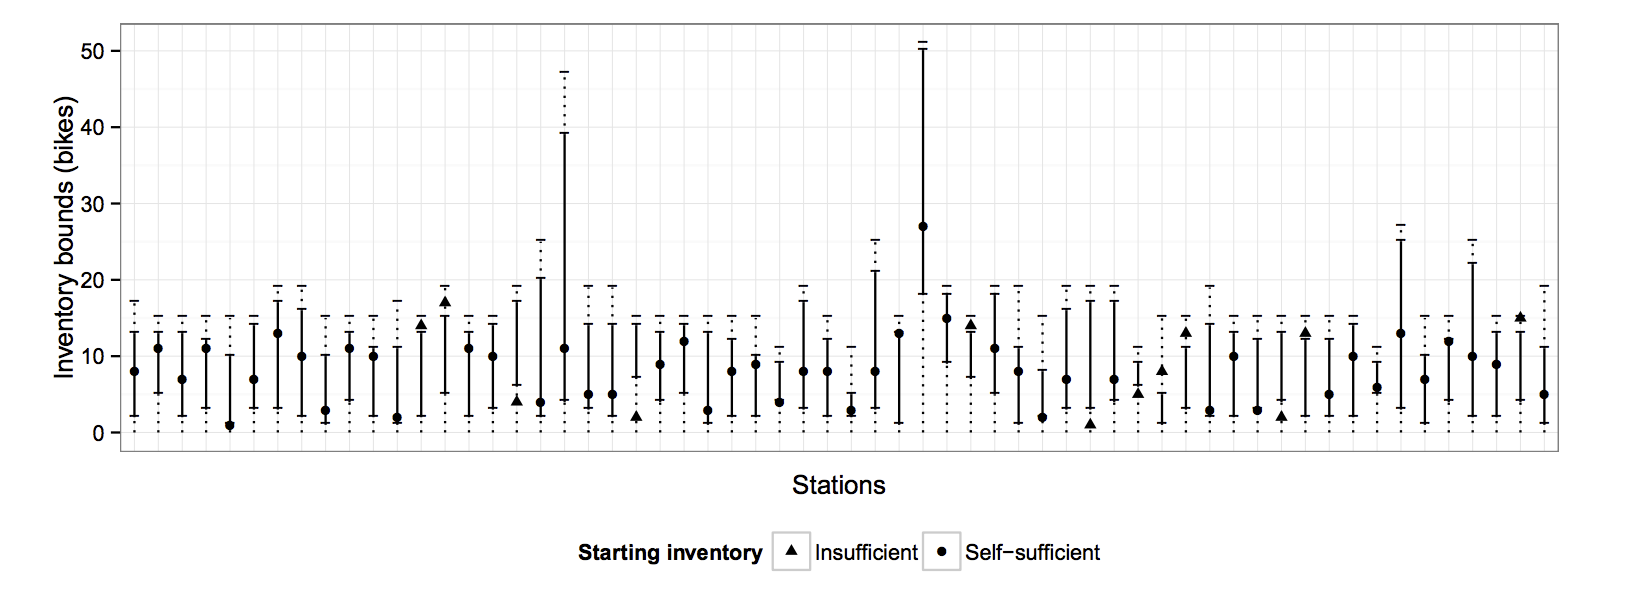
\includegraphics[scale=0.17]{plots/hubway_service_level.png}}
            \caption{Observation period 8--9AM on weekdays with $\beta_i^{-}=\beta_i^{+}=95\%$ on Friday, June 1, 2012\footcite{schuijbroek2017inventory}.}
        \end{figure}
        \pause
        \alert{Authors use Maximum Likelihood Estimator for Poisson variables, but they do not have data for unfulfilled demand!}
    \end{frame}

    \section{Routing Problem for bike-share}
    \begin{frame}{Routing Problem}
    \textbf{Problem (P1):} Given $\mathcal{V}$ re-balancing trucks, each with a capacity of $Q$, re-balance the bike inventory such that service level at each station is met, minimize the maximum tour length of the re-balancing truck to obtain $H^*(\mathcal{S}, \mathcal{V})$. \\
    \vspace{0.2in}
    %\baselineskip
    \pause
    \textbf{Constraints:}
    \begin{itemize}
        \item service level
        \item vehicle and station capacity constraints
        \item flow conservation
        \pause
        \item<alert@3>integrality constraints
    \end{itemize}
    \pause
    \alert{Pure MIP approach: Intractable for realistic scenarios with $|\mathcal{S}| \geq 50$ and $|\mathcal{V}| \geq 3$.}
    \end{frame}

    \section{Clustered Routing Problem}
    \begin{frame}{Clustered Routing Problem}
    \textbf{Problem (P2):} Find a clustering solution that assigns disjoint clusters of stations $\mathcal{S}_v \subseteq \mathcal{S}$ to vehicles
    $v \in \mathcal{V}$ such that the service level requirements can be satisfied using \textit{only} within-cluster vehicle routing. \\
    \pause
    \begin{itemize}
        \item Extended set-partitioning problem.
        \pause
        \item Approximate within-cluster routing costs.
        \pause
        \item<alert@4>{Impose triangle inequality -- within-cluster routing costs lower bounded by length of shortest Hamiltonian path.}
    \end{itemize}
    \pause
    \textbf{Maximum Spanning Star approximation:} \pause $SPS_i(\mathcal{S}_v) = \sum_{j \in \mathcal{S}_v}d_{ij}$.
    \pause
    Maximum-cost spanning star \bigg($\max_{i \in \mathcal{S}_v}SPS_i(\mathcal{S}_v)$\bigg) approximates within-cluster routing cost.
    \end{frame}

    \begin{frame}{Heuristic 1}
    \textbf{Clustered MIP (H1):} \only<2->{\alert{(Sub-optimal)}}
    \begin{enumerate}
        \item Solve (P2)
        \item Solve (P1) for each cluster of stations $\mathcal{S} = \mathcal{S}_v$ and $\mathcal{V} = \{v\}$ to obtain $H^*(\mathcal{S}_v, \{v\})$
        \item $H^* = \max_{v \in \mathcal{V}}H^*(\mathcal{S}_v, \{v\})$
    \end{enumerate}
    \end{frame}
    \begin{frame}{Heuristic 2}
    \textbf{Clustered MIP with Cuts (H2):}
    \begin{enumerate}
        \item Initialize a cut set of stations $\mathcal{C} = \emptyset$
        \item Solve (P2) with additional constraint $\forall v: \mathcal{S}_v \not \subseteq \mathcal{C}$ to obtain $H^*$
        \item Solve (P1) for each cluster of stations $\mathcal{S} = \mathcal{S}_v$ and $\mathcal{V} = \{v\}$ to obtain $H^*(\mathcal{S}_v, \{v\})$
            \begin{itemize}
                \item If $\max_{v \in \mathcal{V}}H^*(\mathcal{S}_v, \{v\}) < H^*$ or $\mathcal{C}=\emptyset$, redefine $H^*$ and store routing solution.
                \item For each $v \in \mathcal{V}$ with $H^*(\mathcal{S}_v, \{v\}) \geq H^*$, redefine $\mathcal{C} = \mathcal{C} \cup \{\mathcal{S}_v\}$ 
            \end{itemize}
        \item Go to step 2.
    \end{enumerate}
    \pause
    \alert{Break sub-optimal clusters by dividing their stations over many different vehicles.}
    \end{frame}

    \begin{frame}{Computation Results for Hubway}
        \begin{figure}
            \centering
            {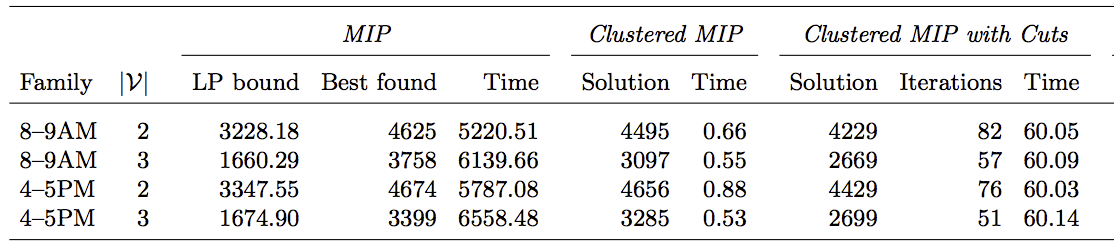
\includegraphics[scale=0.28]{plots/clustered_MIP.png}}
            \caption{Averaged results over 41 runs of algorithms\footcite{schuijbroek2017inventory}.}
        \end{figure}
    \end{frame}

    \begin{frame}{Summary}
    	\textbf{Positives:}
    	\begin{itemize}
    		\item Simple framework for evaluating service level requirements.
    		\item Heuristic algorithm for re-balancing problem in bike-share.
    	\end{itemize}
    		\vspace{0.1in}
    		\pause
    	\textbf{Concerns:}
    	\begin{itemize}
    		\item \alert{Tradeoff between routing costs and revenue loss due to imbalance.}
    		\item \alert{Assumption of negligible demand during the re-balancing operation.}
    	\end{itemize}
    \end{frame}